%%%%%%%%%%%%%%%%%%%%%%%%%%%%%%%%%%%%%%%%%%%%%%%%%%%%%%%%%%%%%%%%%%%%%%%%%%%%
%  第25回 練習問題［50］〜［56］（原本では［45］〜［51］）（旧 prob2_p2.png 〜 prob2_p5.png）
%  ※ このファイルは記録用。実体は physics_ch25.tex に流し込み済み。
%%%%%%%%%%%%%%%%%%%%%%%%%%%%%%%%%%%%%%%%%%%%%%%%%%%%%%%%%%%%%%%%%%%%%%%%%%%%

% 第2巻（prob2_*.png）は原本では［45］から始まるが，第1巻の第24回が［41］〜［49］
% で終わっており原本の側で番号が重複している．ユーザーの指示（2026-09-02）により，
% 第24回からの通し番号になるよう ［50］〜［56］へ振り直した（原本より +5）．
% ※ 第26回以降（原本では［52］始まり）も同じだけずらす必要がある．
\setcounter{qno}{49}

\filbreak
\Rank{A問題}

\Mon{基本公式の確認}

\hspace{1zw}回折格子に対して垂直に波長$600\U{nm}$の単色光を当てたところ，入射方向に対して$30^\circ$の方向に1次の明線が生じた．この回折格子$1\U{m}$あたりの格子の本数は何本か．ただし，空気の絶対屈折率を1とする．

\filbreak
\Rank{B問題}

\Mon[\Sitei]{ヤングの実験}

\begin{zuright}{62mm}
\hspace{1zw}右の図のように，単スリット$\mathrm{A}$，スリット間隔が$d\U{m}$の複スリット$\mathrm{B}$，スクリーン$\mathrm{C}$を用いてヤングの実験を行う．$\mathrm{A}$から$\mathrm{B}$までの距離は$l\U{m}$，$\mathrm{B}$から$\mathrm{C}$までの距離は$L\U{m}$であり，光源は単色（単一の波長のみを出す）である．単スリット$\mathrm{A}$の穴$\mathrm{S_0}$は複スリット$\mathrm{B}$の穴$\mathrm{S_1}$, $\mathrm{S_2}$の垂直二等分線上にある．この垂直二等分線と$\mathrm{C}$との交点を$\mathrm{O}$とし，この点から距離$x\U{m}$だけ離れた点を$\mathrm{P}$点とする．
\zusep
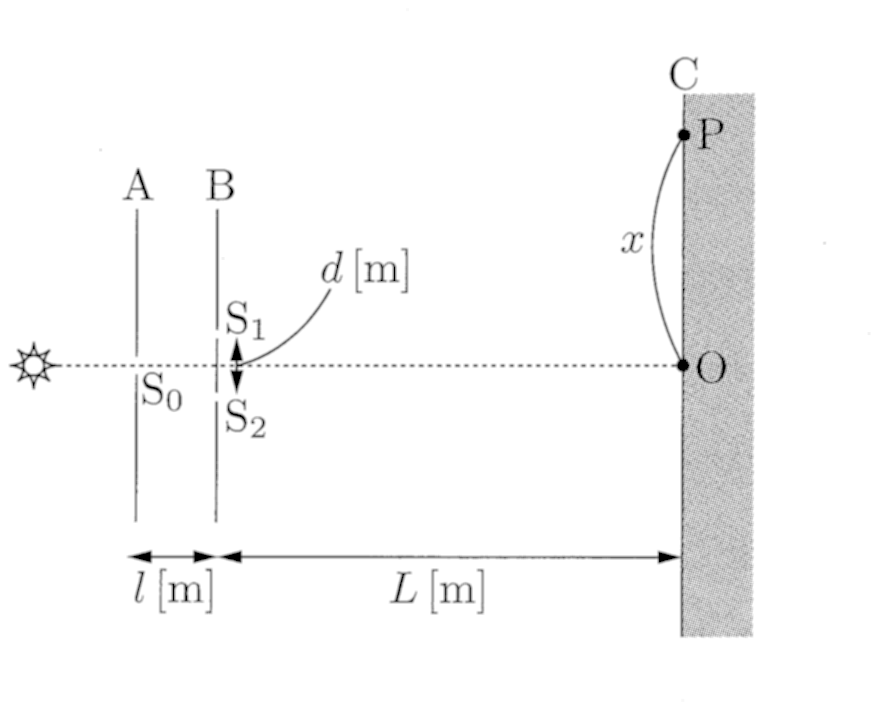
\includegraphics[keepaspectratio,width=62mm]{fig/ch25_p2_young1.png}
\end{zuright}
\hspace{1zw}これについて以下の設問に答えよ．ただし，$x$, $d$は$L$に比べて十分小さいものとし，$|y|\ll 1$に対して成立する近似式$\sqrt{1+y^2}\fallingdotseq 1+\dfrac{1}{2}y^2$を用いてよい．
\begin{komon}
\ko{1} 点$\mathrm{P}$では，$\mathrm{S_0\to S_1\to P}$の経路をたどってくる光と$\mathrm{S_0\to S_2\to P}$の経路をたどってくる光とが干渉する．この二つの光の経路差$\Delta D$を，下の図を参照して三平方の定理を用いて厳密に求めよ．
% 原本は「右の図を参照して」．組版の都合で図を設問の下に置いたため「下の図」に改めた．
       \begin{center}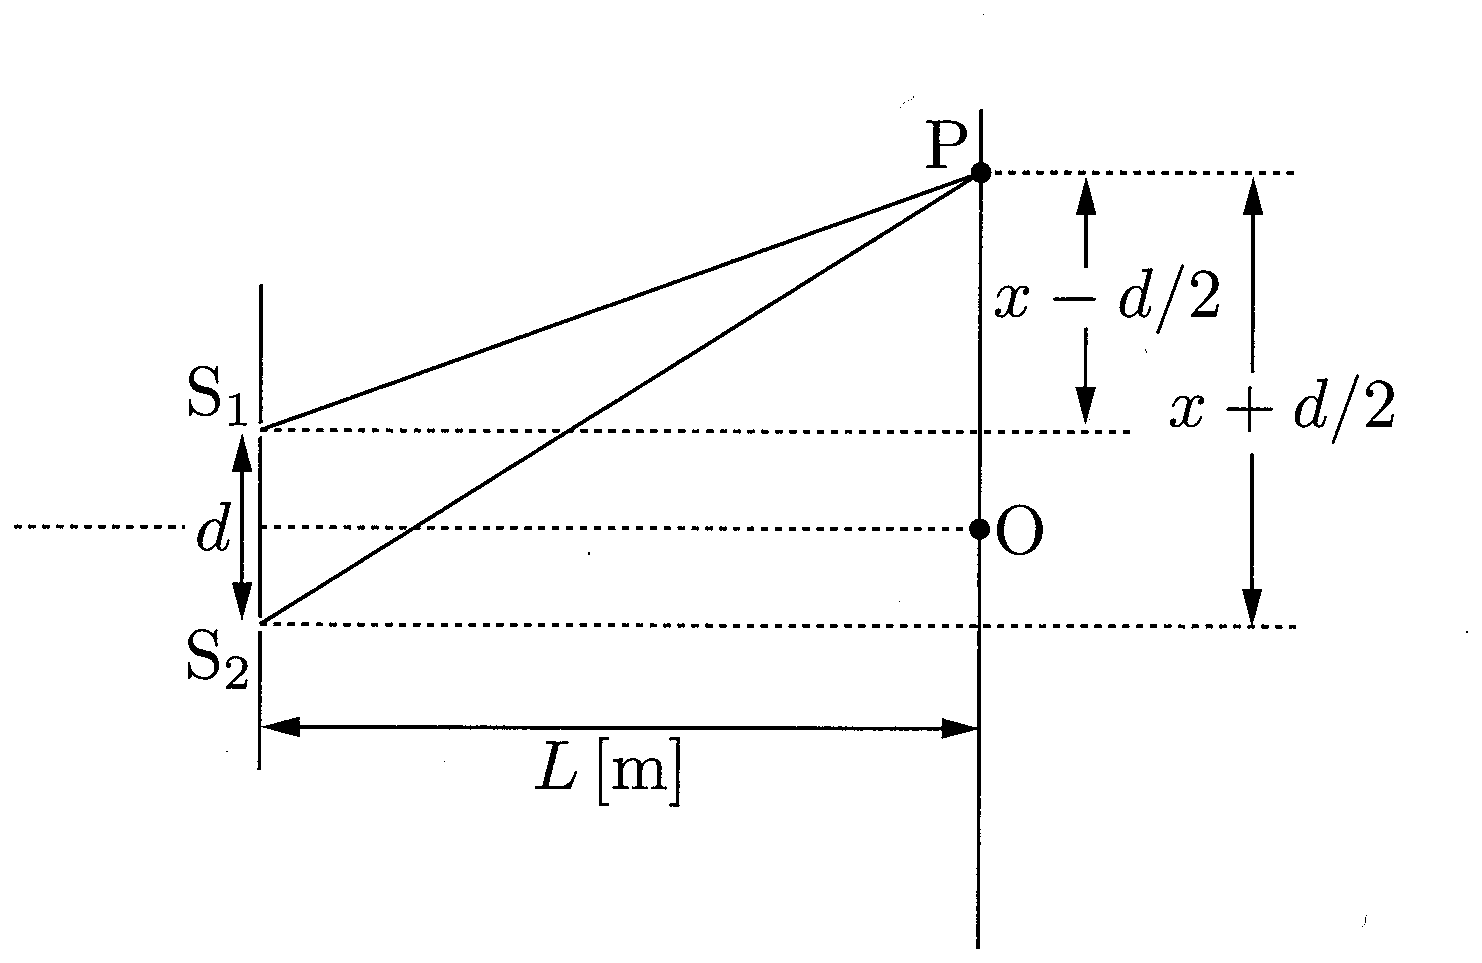
\includegraphics[keepaspectratio,width=76mm]{fig/ch25_p2_young2.png}\end{center}
\ko{2} (1)で求めた経路差$\Delta D$の式を，近似式を用いて一次近似せよ．
\ko{3} 今，スリット幅が$d=0.50\U{mm}$，$\mathrm{B}$と$\mathrm{C}$との距離が$L=1.0\U{m}$であった．実験を行ったところ，スクリーン上には明線が$1.0\U{mm}$の間隔で現れた．このことより，実験に用いた単色光源の波長を求めよ．
\end{komon}

\Mon{光学的距離}

\begin{zuright}{66mm}
\hspace{1zw}波長$\lambda\U{m}$の光源と図のようなスリット間隔$d\U{m}$の複スリットを用いてヤングの実験を行う．ここで，スリット$\mathrm{S_2}$に接触させて屈折率$n$，厚さ$D\U{m}$の十分に薄いガラス$\mathrm{G}$を置き，複スリット$\mathrm{S_1}$, $\mathrm{S_2}$から十分遠方の$L\U{m}$だけ離れたスクリーン上に出来る干渉じまを観察する場合について，以下の設問に答えよ．
\zusep
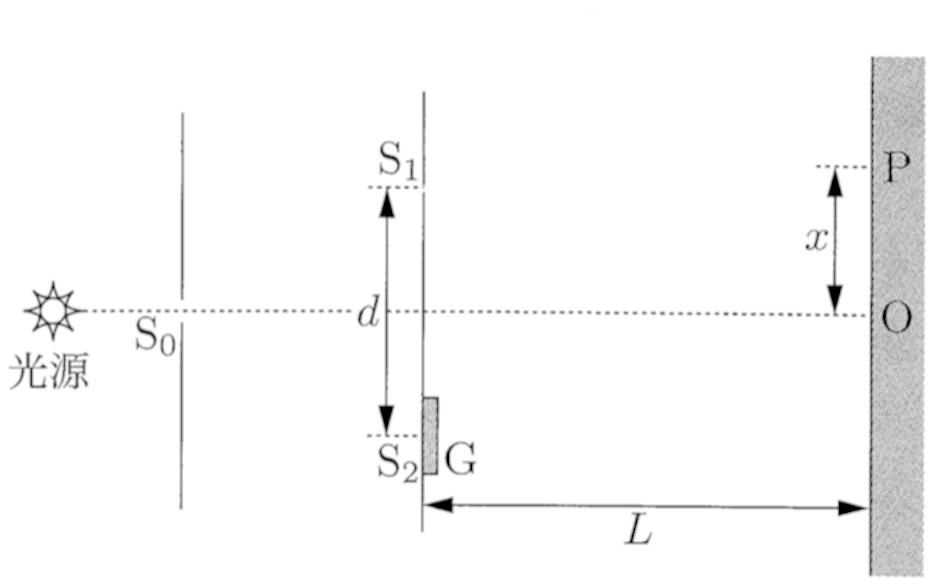
\includegraphics[keepaspectratio,width=66mm]{fig/ch25_p3_glass.png}
\end{zuright}
\hspace{1zw}ただし，$L\gg d$, $x$とし，$\theta$が1より十分小さい場合は，$\sin\theta\fallingdotseq\tan\theta\fallingdotseq\theta$, $\cos\theta\fallingdotseq 1$の近似を用いてよい．空気の絶対屈折率は1であるとする．
\begin{komon}
\ko{1} ガラス$\mathrm{G}$がない場合には，図の$\mathrm{P}$点に入射してくる二つの光はどれだけの光路差を持っているか．$\mathrm{S_2}$を経由してくる光の光路の方が長い場合を正として答えよ．
\ko{2} 実際に図の$\mathrm{P}$点にやってくる二つの光は，ガラス$\mathrm{G}$があるためにさらに光路差を生じている．スリット$\mathrm{S_2}$を出た光はガラス$\mathrm{G}$に対してほぼ垂直に入射することに注意して，ガラス$\mathrm{G}$を置くことによって新たに生じる光路差はいくらか．$\mathrm{S_2}$を経由してくる光の光路の方が長い場合を正として答えよ．
\ko{3} 以上より，二つのスリットから$\mathrm{P}$点にやってくる二つの光が強め合うための条件を整数$m$を用いて表し，さらにスクリーン上に出来る明線の間隔を求めよ．
\end{komon}

\Mon[\Sitei]{回折格子}

\begin{zuright}{58mm}
\hspace{1zw}小さいガラス板$\mathrm{R}$の表面に溝（格子線）を間隔$d\U{m}$で等間隔に多数刻んで作った回折格子がある．図のように$\mathrm{R}$に垂直に平行光線を当て，格子線に垂直な平面内で入射方向から角度$\theta$の方向に回折する光線$\mathrm{L}$を調べる．$\mathrm{R}$から十分遠方に入射光線に垂直にスクリーン$\mathrm{T}$を置き，回折光$\mathrm{L}$が$\mathrm{T}$に当たるところにスリット$\mathrm{S}$を設ける．以下の問に答えよ．
\zusep
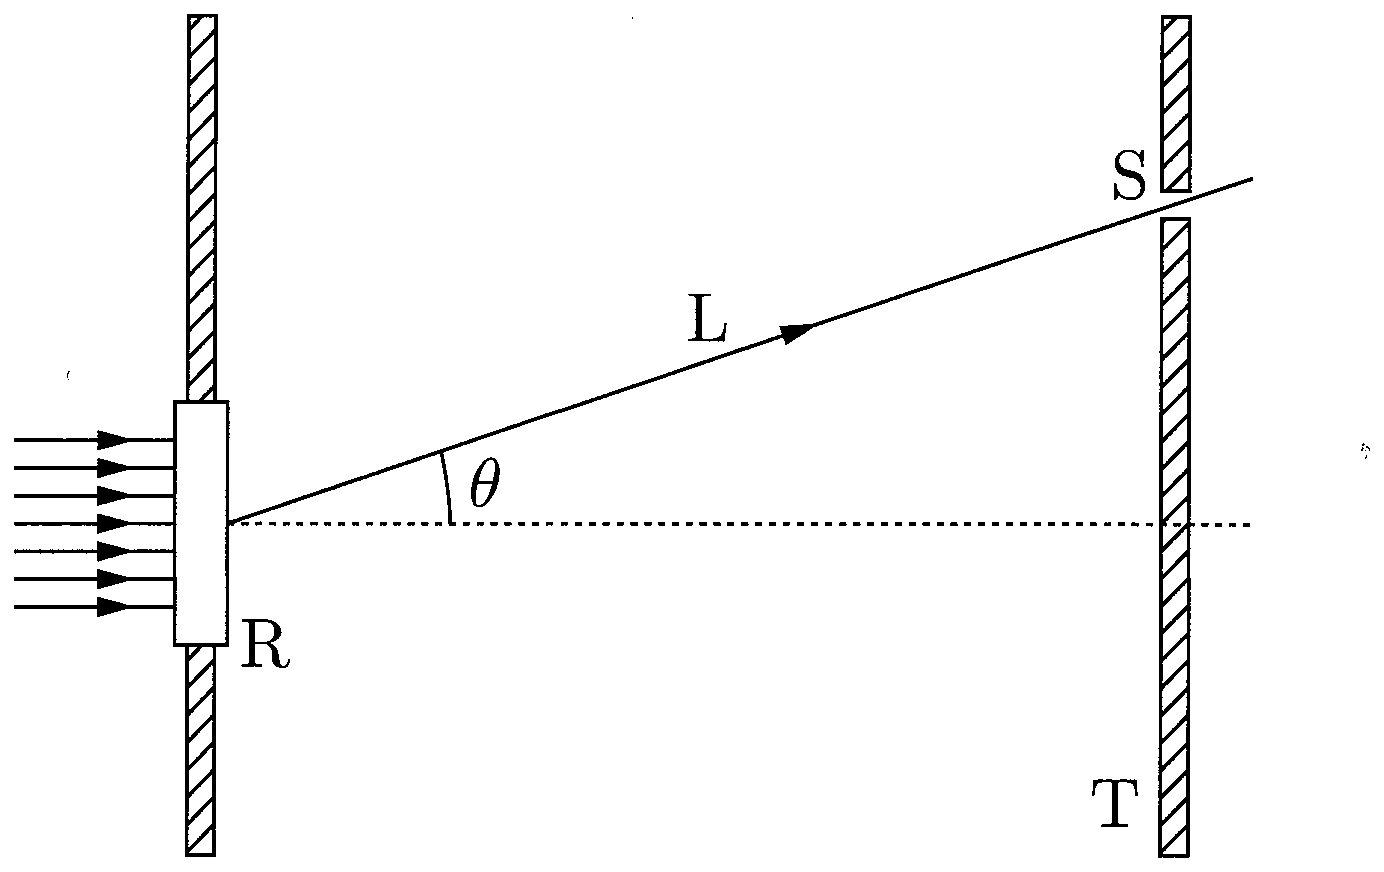
\includegraphics[keepaspectratio,width=58mm]{fig/ch25_p3_grating.png}
\end{zuright}
\begin{komon}
\ko{1} 波長$\lambda\U{m}$の光をガラス板$\mathrm{R}$に入射する．このとき，スリット$\mathrm{S}$のところに明線が生じるために必要な，$d$, $\theta$, $\lambda$が満たすべき条件式を示せ．
\ko{2} ガラス板$\mathrm{R}$上に$1.0\U{mm}$当たり250本の格子線がある．白色光（$380\U{nm}$〜$780\U{nm}$の範囲のすべての波長の光を含む光）を$\mathrm{R}$に当てる．このとき角度$\theta=30^\circ$方向で明線となる光の波長をすべて求めよ．
\end{komon}

\filbreak
\Rank{C問題}

\Mon{ロイドの鏡}

\begin{zuright}{66mm}
\hspace{1zw}波長$\lambda\U{m}$の単色光源$\mathrm{P}$，単スリット$\mathrm{S}$，鏡$\mathrm{M}$の三つを右図のように配置し，光源$\mathrm{P}$を点灯させてスリットから十分遠方の距離$L\U{m}$の位置にスクリーンを置くと，スクリーン上にはヤングの実験とほとんど同様な干渉縞が観測される．この実験に関して，$L\gg x$, $d$として以下の設問に答えよ．
\zusep
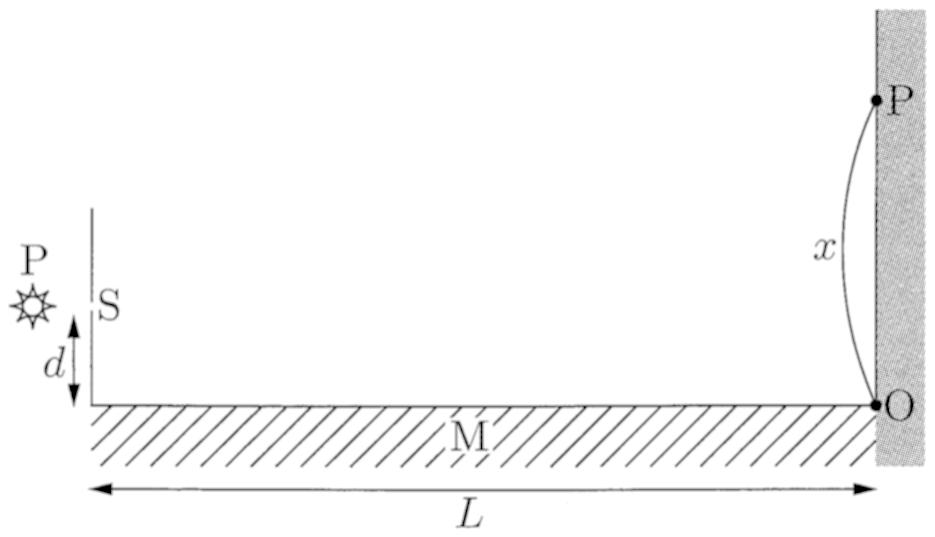
\includegraphics[keepaspectratio,width=66mm]{fig/ch25_p4_lloyd.png}
\end{zuright}
\begin{komon}
\ko{1} スクリーン上に干渉縞が観察されるのは，二つの経路でやってくる光が互いに強め合い・弱め合いを起こすためである．この二つの経路とはどのような経路か．
\ko{2} スクリーン上の$\mathrm{O}$点から距離$x\U{m}$の$\mathrm{P}$点にやってくる二つの光の経路差を，図中の$d$, $L$および$x$を用いて表せ．ただし，微小量$|\theta|\ll 1$に対して成立する近似式$\sin\theta\fallingdotseq\tan\theta\fallingdotseq\theta$, $\cos\theta\fallingdotseq 1$を利用せよ．
\ko{3} スクリーン上に明線が出来る座標$x$を，自然数$m$を用いて表し，さらに明線間隔を求めよ．
\end{komon}

\Mon{光速の測定実験（フーコーの実験）}

\begin{zuright}{58mm}
\hspace{1zw}以下の文は光速の測定に関する実験（フーコーの実験）について述べたものである．文中の空欄\framebox[3zw]{\rule{0pt}{1.1zw}}の中に当てはまる適当な式および数値を答えよ．

\hspace{1zw}フーコーは，右図のように固定鏡と高速で回転する鏡を用いて光の速さを測定した．光源$\mathrm{S}$から出た光が回転鏡$\mathrm{R}$で反射されたのち，図のように固定鏡$\mathrm{M}$で反射されて回転鏡$\mathrm{R}$に戻ってくるまでに，回転鏡が$\theta\U{rad}$だけ回転したとすると，
\zusep
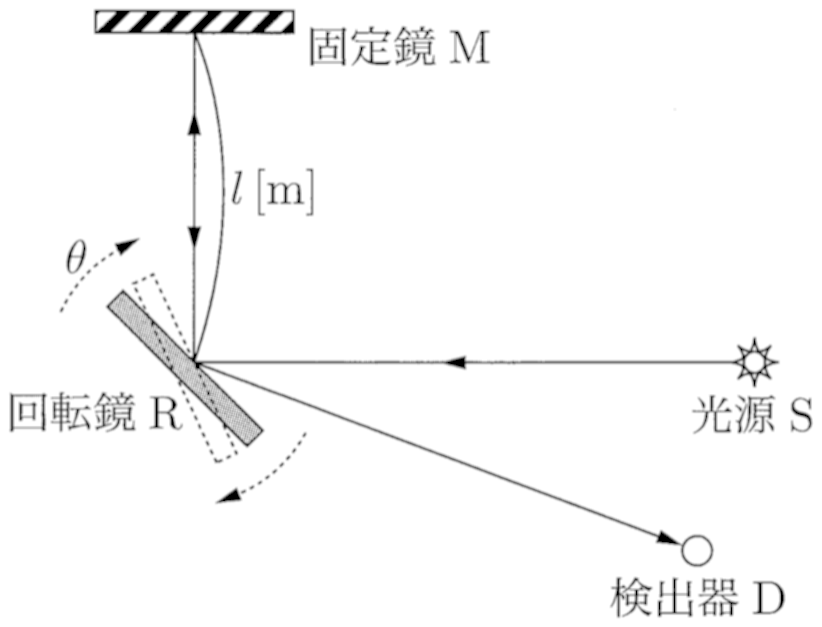
\includegraphics[keepaspectratio,width=58mm]{fig/ch25_p4_foucault.png}
\end{zuright}
再び$\mathrm{R}$で反射した光の進行方向$\mathrm{RD}$は元の光源の方向（$\mathrm{RS}$の方向）より下向きに角度\fbox{\MARU{1}}だけ振れた方向になる．今，固定鏡と回転鏡の距離を$l\U{m}$，回転鏡の回転数を$N\,[回/\mathrm{s}]$とすると，回転鏡が$\theta\U{rad}$だけ回転するのに要する時間は\fbox{\MARU{2}}である．一方，光の速さを$c\U{m/s}$とすると，回転鏡と固定鏡の間を光が往復するのに要する時間は\fbox{\MARU{3}}である．回転に要する時間と回転鏡と固定鏡の間を光が往復するのに要する時間とは等しいから，光の速さは\fbox{\MARU{4}}となる．フーコーの実験では，$l=20.0\U{m}$, $N=800\,[回/\mathrm{s}]$のとき$\theta=6.73\times 10^{-4}\U{rad}$であった．よって光の速さは\fbox{\MARU{5}}となる．

\Mon{ヤングの実験}

\begin{zuright}{60mm}
\hspace{1zw}複スリット$\mathrm{A}$, $\mathrm{B}$を持った板$\mathrm{F}$の左方で，$\mathrm{A}$, $\mathrm{B}$から等距離の位置に単スリットおよび光源があり，$\mathrm{F}$の右方にはスクリーン$\mathrm{W}$が置かれている．複スリット$\mathrm{A}$, $\mathrm{B}$の幅は単色光源の波長$\lambda\U{m}$に比べて十分に小さく，複スリットの間隔$2d\U{m}$は波長の数倍以上の大きさである．単スリットから$\mathrm{F}$までの距離は$L\U{m}$，$\mathrm{F}$から$\mathrm{W}$までの距離は$l\U{m}$で，$L$, $l$は$2d$に比べて十分大きい．
\zusep
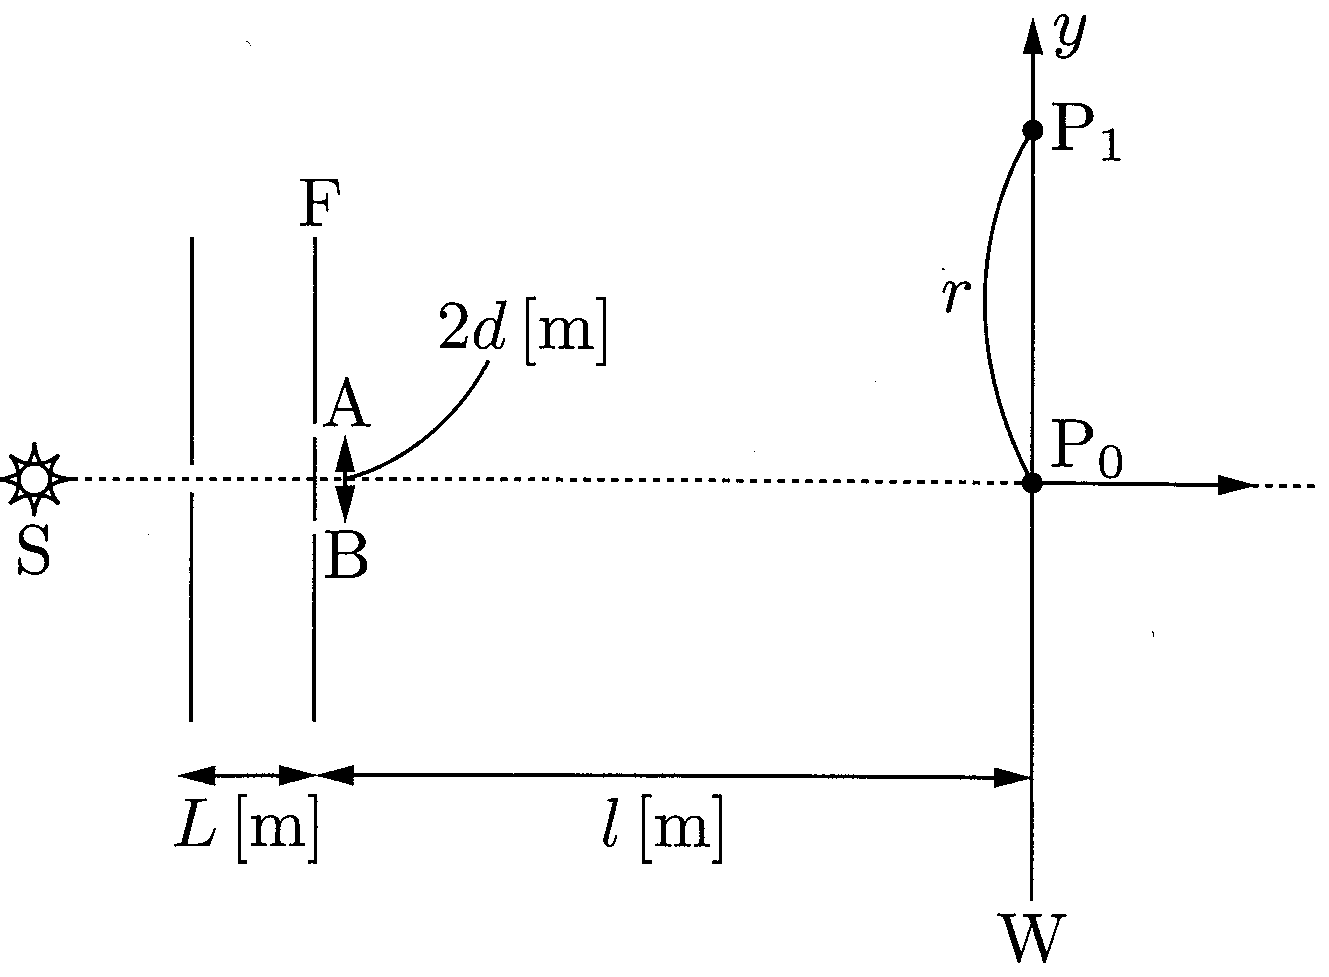
\includegraphics[keepaspectratio,width=60mm]{fig/ch25_p5_young.png}
\end{zuright}
\hspace{1zw}これについて，以下の設問に答えよ．ただし，微小量$|\varepsilon|\ll 1$に対して成り立つ近似式$(1+\varepsilon)^n\fallingdotseq 1+n\varepsilon$を用いてよい．
\begin{komon}
\ko{1} 複スリットを通った光は，スクリーン上に図に示すような強度分布の干渉縞を生じた．最も明るい線$\mathrm{P_0}$と隣の明るい線$\mathrm{P_1}$との間隔は$r\U{m}$である．$\lambda$と$r$の関係式を求めよ．
       \begin{center}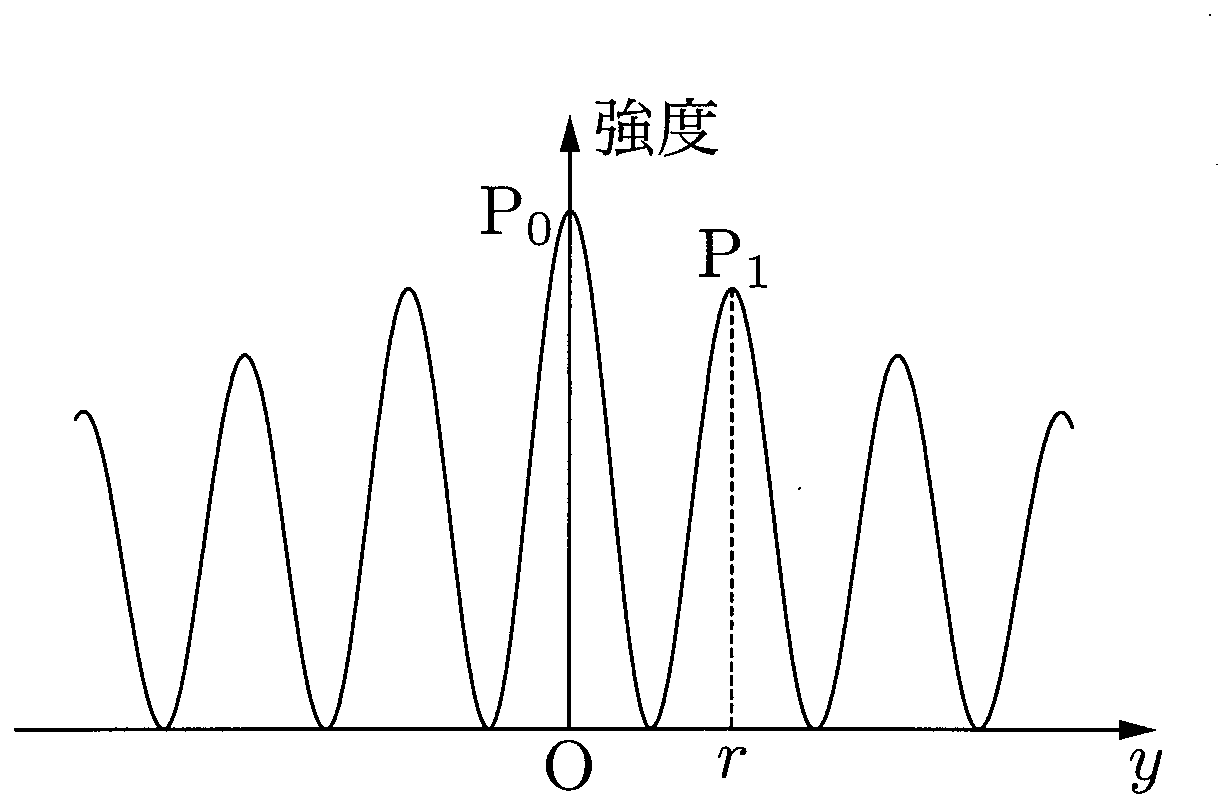
\includegraphics[keepaspectratio,width=76mm]{fig/ch25_p5_int.png}\end{center}
\ko{2} 単スリットを$y$軸の正方向へ距離$y_0\U{m}$だけ移動させると，スクリーン上の最も明るい線$\mathrm{P_0}$はどちらへどれだけ移動するか．ただし，$y_0\U{m}$も十分小さいものとする．
\ko{3} $\mathrm{S}$を初めの位置に戻し，$\mathrm{W}$を右方へ距離$x\U{m}$だけ動かすと，$\mathrm{P_1}$はどちらへどれだけ移動するか．
\end{komon}
